\documentclass[12pt, twoside]{article}
\usepackage[letterpaper, margin=1in, headsep=0.5in]{geometry}
\usepackage[english]{babel}
\usepackage[utf8]{inputenc}
\usepackage{amsmath}
\usepackage{amsfonts}
\usepackage{amssymb}
\usepackage{tikz}
\usepackage{yhmath}
\usetikzlibrary{quotes, angles}
\usepackage{graphicx}
\usepackage{enumitem}
\usepackage{multicol}

\newif\ifmeta
\metatrue %print standards and topics tags

\title{Regents Geometry}
\author{Chris Huson}
\date{April 2022}

\usepackage{fancyhdr}
\pagestyle{fancy}
\fancyhf{}
\renewcommand{\headrulewidth}{0pt} % disable the underline of the header
\raggedbottom

\fancyhead[LE]{\thepage}
\fancyhead[RO]{\thepage \\ Name: \hspace{4cm} \,\\}
\fancyhead[LO]{BECA / Dr. Huson / Geometry\\* Unit 11: Function transformations\\* 27 April 2022}

\begin{document}
\subsubsection*{11.3 Square root function \hfill HSF.BF.B.3}
\begin{enumerate}
\item The parabola with the equation $y-1=(x-2)^2$, is shown below. 
\begin{multicols}{2}
  \begin{enumerate}
    \item What translation would map $V(2,1) \rightarrow (0,0)$?\vspace{2cm}
    \item Reflect the parabola across the $y$-axis.
    \item Mark and label the image $V'$ with its coordinates. \vspace{2cm}
  \end{enumerate}
  \begin{flushright}
    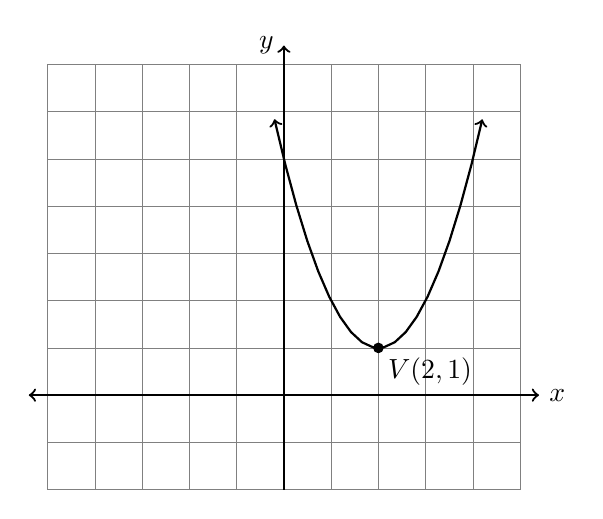
\begin{tikzpicture}[scale=0.6]
    \draw [help lines] (-5,-2) grid (5,7);
    \draw [thick, <->] (-5.4,0) -- (5.4,0) node [right] {$x$};
    \draw [thick, ->] (0,-2)--(0,7.4) node [left] {$y$};  
    \draw [thick,<->,samples=20,domain=-0.2:4.2] plot(\x,{(\x-2)^2+1});
    \draw [fill] (2,1) circle [radius=0.1] node[below right] {$V(2,1)$};
  \end{tikzpicture}
\end{flushright}
\end{multicols}

\item The line $l$ having the equation $\displaystyle y-2=-\frac{2}{3}(x-3)$ is shown below.
\begin{multicols}{2}
  \begin{enumerate}
    \item Write down coordinates of $P$.
    \item Point $P$ is mapped to the origin by\\ $x \rightarrow x-h$\\ $y \rightarrow y-k$ \\Write down $h$ and $k$.
    \item Plot the image of $l$ after the translation.
  \end{enumerate}
  \begin{flushright}
    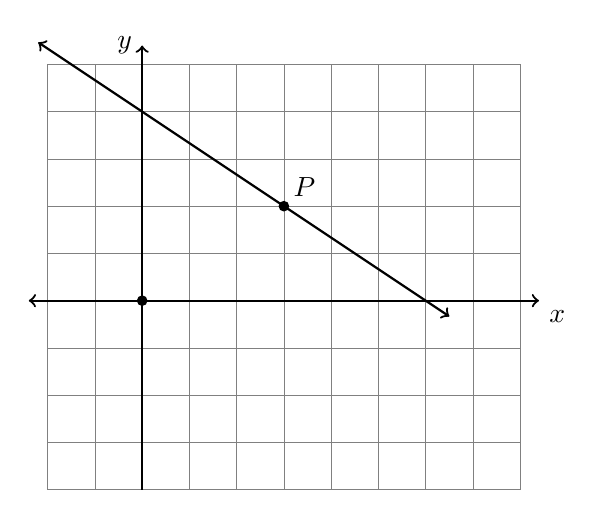
\begin{tikzpicture}[scale=0.6]
      \draw [help lines] (-2,-4) grid (8,5);
      \draw [thick, <->] (-2.4,0) -- (8.4,0) node [below right] {$x$};
      \draw [thick, ->] (0,-4.0)--(0,5.4) node [left] {$y$};
      \draw [thick,<->,samples=20,domain=-2.2:6.5] plot(\x,-2/3*\x+4);
      \draw [fill] (3,2) circle [radius=0.1] node[above right] {$P$};
      \draw [fill] (0,0) circle [radius=0.1];
    \end{tikzpicture}
  \end{flushright}
\end{multicols}%\vspace{1cm}

\item The parabola $y+1=(x-2)^2$ graphed below.
\begin{multicols}{2}
\begin{enumerate}
  \item Write down its $y$-intercept.
  \item Write down its $x$-intercepts.
  \item Reflect $f$ across the $y$-axis.
  \item Mark and label the image\\ parabola's intercepts and vertex.
\end{enumerate}
\begin{center} 
\begin{tikzpicture}[xscale=1, yscale=1]
  \draw [thick, ->] (-3.2,0) -- (5.4,0) node [above left] {$x$};
  \draw [thick, ->] (0,-0.5)--(0,4.4) node [left] {$y$};
  \foreach \x in {-3,-2,-1,1,2,3,4, 5} \draw (\x cm,3pt)--(\x cm,-3pt) node[below] {$\x$};
  \foreach \y in {1,2,3} \draw (3pt,\y cm)--(-3pt,\y cm) node[left] {$\y$};
  \draw [thick,<->,samples=40,domain=-0.25:4.25] plot(\x,{(\x-2)^2-1});
  \fill (2,-1) circle[radius=0.08];
  \node at (2.5,-1.5){$(2,-1)$};
  \node at (4.5,3){$f(x)$};
\end{tikzpicture}
\end{center}
  \end{multicols}

\newpage
Definition: The \emph{square root} of a real number $x$ is the number $y$ such that $y^2=x$. For example, 3 is the square root of 9 because $3^2=9$. \\[0.25cm]
In general, there is a positive and a negative square root, $(-3)^2=9$ also. The positive square root is called the \emph{principal square root} and written with the radical sign: $\sqrt{9}=3$. To represent both the positive and negative square roots we write $\pm \sqrt{\quad}$

\item Complete the t-table for the function $f$: $y=\sqrt{x}$, plot the points, and draw $f$ as a smooth curve.
  \begin{center} 
  \begin{tikzpicture}[scale=0.8]
    \draw [help lines] (-1,-1) grid (10,5);
    \draw [thick, ->] (-1.2,0) -- (10.4,0) node [below right] {$x$};
    \draw [thick, ->] (0,-0.2)--(0,5.4) node [right] {$y$};
    \foreach \x in {0,1,2,...,10} \draw (\x cm,1pt)--(\x cm,-1pt) node[below] {$\x$};
    \foreach \y in {1,2,3,4,5} \draw (1pt,\y cm)--(-1pt,\y cm) node[left] {$\y$};
    \draw [thick] (-7,-3) -- (-7,6);
    \draw [thick] (-8.5,5) -- (-5.5,5);
    %\node at (-7,7){$f(x)$};
    \node at (-8,5.5){$x$}; \node at (-6,5.5){$\sqrt{x}$};
    \node at (-8,4){$0$}; \node at (-6,4){$0$};
    \node at (-8,2.5){$1$}; 
    \node at (-8,1){$4$};
    \node at (-8,-0.5){$9$};\node at (-6,-0.5){$3$};
    \fill (0,0) circle[radius=0.1];
    %\fill (1,1) circle[radius=0.1];
    \fill (9,3) circle[radius=0.1];
  \end{tikzpicture}
  \end{center}

\item The function $g: y = \sqrt{x-1}+2$ is plotted below as a solid line. What translation would map $g$ onto the parent function (dotted)?  State your answer in the form $x \rightarrow x-h$, $y \rightarrow y-k$.
\begin{center} 
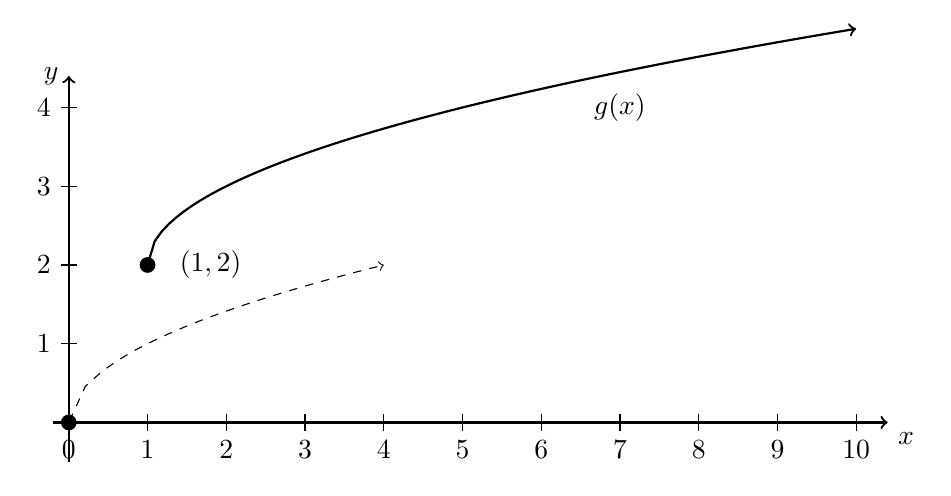
\begin{tikzpicture}[xscale=1.0, yscale=1]
  \draw [thick, ->] (-0.2,0) -- (10.4,0) node [below right] {$x$};
  \draw [thick, ->] (0,-0.5)--(0,4.4) node [left] {$y$};
  \foreach \x in {0,1,2,...,10} \draw (\x cm,3pt) -- (\x cm,-3pt) node[below] {$\x$};
  \foreach \y in {1,2,3,4} \draw (3pt,\y cm) -- (-3pt,\y cm) node[left] {$\y$};
  \draw [dashed,<->,samples=20,domain=0:4] plot(\x,\x^0.5);
  \fill (0,0) circle[radius=0.1];
  \draw [thick,->,samples=100,domain=1:10] plot(\x,{(\x-1)^0.5+2});
  \fill (1,2) circle[radius=0.1];
  \node at (1.8,2){$(1,2)$};
  \node at (7,4){$g(x)$};
\end{tikzpicture}
\end{center}

\end{enumerate}
\end{document}
  